\chapter{Càlculs Bàsics}\label{sec:calc_bas}

\section{Introducció}
Es tracten en aquest capítol càlculs bàsics que poden utilitzar-se en la
resolució de diversos problemes electrotècnics.



\section{Càlculs en per unitat} \label{sec:seccio_pu} \index{pu}\index{per unitat}

Les magnituds expressades en «pu» (per unitat) són útils quan es treballa
amb xarxes de corrent altern on hi ha transformadors, i per tant més d'un nivell de tensió.

\subsection{Mètode de càlcul} \index{pu!mètode de càlcul}

\index{pu!magnituds base fonamentals} El primer pas consisteix en
escollir unes magnituds base. Les magnituds base fonamentals són la
potència i la tensió; s'escull una potència base $S\ped{B}$ per a
tota la xarxa, i tantes tensions base $U_{\text{B}_1}, U_{\text{B}_2}, \ldots,
U_{\text{B}_n}$ com nivells de tensió
diferents tingui la xarxa:
\begin{equation}
   \text{Magnituds base fonamentals:}\;\left\{
\begin{array}{l}
   S\ped{B} \\
   U_{\text{B}_1}, U_{\text{B}_2}, \ldots, U_{\text{B}_n}
\end{array}
\right.
\end{equation}

Normalment s'escull com a tensions base les tensions nominals dels transformadors de la
xarxa, i com a potència base la potència nominal d'un del transformadors o generadors de la xarxa; també és usual utilitzar com a potència base el valor \SI{100}{MVA}.

En el cas de circuits monofàsics, les tensions base són les tensions monofàsiques, o fase--neutre $U\ped{FN}$, i la potència base és la potència monofàsica $S\ped{1F}$. En el cas de circuits trifàsics, podem escollir com a tensions base les tensions fase--neutre $U\ped{FN}$ i com a potència base la potència  monofàsica $S\ped{1F}$, o bé podem escollir com a tensions base les tensions fase--fase $U\ped{FF}$ i com a potència base la potència trifàsica $S\ped{3F}$.

\index{pu!magnituds base}A partir de la potència base i de les tensions base es
defineixen els corrents base $I_{\text{B}_i}$, les impedàncies base $Z_{\text{B}_i}$ i les
admitàncies base $Y_{\text{B}_i}$. Segons que s'utilitzin les tensions i potències monofàsiques o trifàsiques com a magnituds base, tenim:
\begin{equation}
\begin{array}{c}  S\ped{B}=S\ped{1F} \\ U_{\text{B}_i} = U_{\text{FN}_i} \\ (i=1,\ldots,n) \end{array}
\left\{
\begin{array}{l}
   I_{\text{B}_i} = \dfrac{S\ped{B}}{U_{\text{B}_i}} \\[2.5ex]
   Z_{\text{B}_i} = \dfrac{U_{\text{B}_i}^2}{S\ped{B}} = \dfrac{U_{\text{B}_i}}{I_{\text{B}_i}} \\[2.5ex]
   Y_{\text{B}_i} = \dfrac{S\ped{B}}{U_{\text{B}_i}^2} = \dfrac{I_{\text{B}_i}}{U_{\text{B}_i}}
\end{array}
\right.
\qquad\qquad
\begin{array}{c} S\ped{B}=S\ped{3F} \\ U_{\text{B}_i} = U_{\text{FF}_i} \\ (i=1,\ldots,n) \end{array}
\left\{
\begin{array}{l}
   I_{\text{B}_i} = \dfrac{S\ped{B}}{\sqrt{3} U_{\text{B}_i}} \\[2.5ex]
   Z_{\text{B}_i} = \dfrac{U_{\text{B}_i}^2}{S\ped{B}}= \dfrac{U_{\text{B}_i}}{\sqrt{3} I_{\text{B}_i}} \\[2.5ex]
   Y_{\text{B}_i} = \dfrac{S\ped{B}}{U_{\text{B}_i}^2} = \dfrac{\sqrt{3} I_{\text{B}_i}}{U_{\text{B}_i}}
\end{array}
\right.
\label{eq:bases_pu}
\end{equation}

Les magnituds expressades en per unitat (escrites usualment en minúscules) s'obtenen
dividint les magnituds reals (escrites usualment en majúscules) pels valors base corresponents:
\begin{equation}
   \cmplx{s} = \frac{\cmplx{S}}{S\ped{B}} \qquad \cmplx{u} = \frac{\cmplx{U}}{U\ped{B}} \qquad \cmplx{i} = \frac{\cmplx{I}}{I\ped{B}} \qquad \cmplx{z} = \frac{\cmplx{Z}}{Z\ped{B}} \qquad \cmplx{y} = \frac{\cmplx{Y}}{Y\ped{B}}
\end{equation}

Quan es tracta de resoldre circuits trifàsics equilibrats fem servir sempre els circuits equivalents per fase, i podem escollir aleshores com a valors base per a la potència i la tensió, la potència monofàsica $S\ped{1F}$ i la tensió fase--neutre $U\ped{FN}$ respectivament, o la potència trifàsica $S\ped{3F}$ i la tensió fase--fase $U\ped{FF}$ respectivament.


 Quan fem la reducció de valors reals a valors en per unitat, hem de ser conseqüents i utilitzar sempre les potències monofàsiques i les tensions fase--neutre en el primer cas, i les potències trifàsiques i les tensions fase--fase en el segon cas.

 Donat que es verifica $S\ped{3F}=3 S\ped{1F}$ i $U\ped{FF}=\sqrt{3}U\ped{FN}$, els valors  del corrent base $I\ped{B}$, de la impedància base $Z\ped{B}$ i  de l'admitància base $Y\ped{B}$ són els mateixos, tant si utilitzem $S\ped{B}=S\ped{1F}$ i $U\ped{B}=U\ped{FN}$, com si utilitzem $S\ped{B}=S\ped{3F}$ i $U\ped{B}=U\ped{FF}$.

 En ambdós casos $I\ped{B}$ i $\cmplx{I}$ són corrents fase--neutre, $Z\ped{B}$ i $\cmplx{Z}$ són impedàncies fase--neutre i $Y\ped{B}$ i $\cmplx{Y}$ són admitàncies fase--neutre; si tenim càrregues connectades en triangle caldrà transformar-les en càrregues equivalents connectades en estrella per tal de poder aplicar aquest mètode (vegeu la secció \ref{secc:d_y}).

El pas següent consisteix en representar el circuit equivalent en
per unitat i resoldre'l; en el cas de circuits trifàsics, i com a conseqüència del procés utilitzat, el circuit equivalent en per unitat és un circuit monofàsic i com a tal l'hem de resoldre, és a dir, sense la intervenció del factor $\sqrt{3}$.

Un cop resolt el circuit, es multipliquen les magnituds obtingudes en per unitat pels
seus valors base respectius, per tal d'obtenir les magnituds reals:
\begin{equation}
   \cmplx{S} = \cmplx{s} S\ped{B} \qquad \cmplx{U} = \cmplx{u} U\ped{B} \qquad \cmplx{I} = \cmplx{i} I\ped{B} \qquad \cmplx{Z} = \cmplx{z} Z\ped{B} \qquad \cmplx{Y} = \cmplx{y} Y\ped{B}
\end{equation}

\subsection{Canvi de base}\label{sec:canvi-base} \index{pu!canvi de base}

Normalment les impedàncies de transformadors (impedància de curtcircuit) o de generadors (impedància sincrònica, transitòria, etc.) estan referides a les magnituds nominals de la màquina en qüestió.


Si les magnituds base escollides coincideixen amb les nominals de la màquina,
la impedància de la màquina en qüestió estarà expressada ja directament en per unitat, respecte aquesta base.

 En canvi si les magnituds base són diferents de les nominals de la màquina, caldrà fer un canvi de base per tal de referir la impedància de la màquina a les magnituds base escollides.

De forma genèrica, si $\cmplx{z}$ és una impedància referida a la base $U\ped{B}$ i $S\ped{B}$, podem obtenir la impedància $\cmplx{z}'$ referida a la base $U_{\text{B}'}$ i $S_{\text{B}'}$, mitjançant el canvi:
\begin{equation}
   \cmplx{z}' = \cmplx{z} \; \frac{Z\ped{B}}{Z\ped{B}'} = \cmplx{z} \; \frac{U\ped{B}^2}{U_{\text{B}'}^2} \; \frac{S_{\text{B}'}}{S\ped{B}}\label{eq_pu_canvi_base}
\end{equation}

\addcontentsxms{Aplicació del mètode de càlcul en per unitat}
\begin{exemple}[Aplicació del mètode de càlcul en per unitat]\label{ex:cc-pu}
    Es tracte de calcular el corrent de curtcircuit trifàsic en el punt F de la xarxa següent, suposant
    que el sistema està treballant en buit.
    \begin{center}
        \input{Imatges/Cap-CalcBas-pu-Circuit1.pdf_tex}
    \end{center}

    Les dades del generador G, del transformador T1, de la línia L i del transformador T2 són:
    \begin{align*}
       S\ped{G} &= \SI{60}{MVA} & S\ped{T1} &= \SI{40}{MVA} & l\ped{L} &= \SI{22}{km} & S\ped{T2} &=
       \SI{12}{MVA} \\
       U\ped{G} &= \SI{10,5}{kV} & m\ped{T1} &= \SI{10,5}{kV}\!:\!\SI{63}{kV} & U\ped{L} &= \SI{60}{kV} & m\ped{T2} &= \SI{60}{kV}\!:\!\SI{10,5}{kV} \\
       X''\ped{G} &= \SI{12}{\percent} & X\ped{T1} &= \SI{10}{\percent} & X\ped{L} &= \SI{0,4}{\ohm/km} & X\ped{T2} &= \SI{8}{\percent}
    \end{align*}

    Escollim en primer lloc les següents magnituds base: $S\ped{B} = \SI{60}{MVA}$ i $U\ped{B}
    = \SI{10,5}{kV} / \SI{63}{kV} / \SI{10,5}{kV}$.

    Calculem a continuació els valors en per unitat dels diferents elements de la xarxa:

    \textbf{Generador}. En coincidir les magnituds base amb les nominals del generador tenim
     directament:
    \[
    x''\ped{G} = \SI{0,12}{pu}
    \]

    \textbf{Transformador 1}. La relació de transformació i la reactància són respectivament:
    \begin{align*}
    m\ped{T1} &= \frac{\SI{10,5}{kV}}{\SI{10,5}{kV}} :
    \frac{\SI{63}{kV}}{\SI{63}{kV}} = 1\!:\!1 \\[3mm]
    x\ped{T1} &= \num{0,10} \times \frac{(\SI{63}{kV})^2}{(\SI{63}{kV})^2} \times
    \frac{\SI{60}{MVA}}{\SI{40}{MVA}}  = \SI{0,15}{pu}
    \end{align*}

    \textbf{Línia}. La reactància és:
    \[
    x\ped{L} = \frac{\SI{0,4}{\ohm/km} \times \SI{22}{km}} {\dfrac{(\SI{63}{kV})^2}{\SI{60}{MVA}}}  =
    \SI{0,1330}{pu}
    \]

    \textbf{Transformador 2}. La relació de transformació i la reactància són respectivament:

    \begin{align*}
    m\ped{T2} &= \frac{\SI{60}{kV}}{\SI{63}{kV}} :
    \frac{\SI{10,5}{kV}}{\SI{10,5}{kV}} = \num{0,9524}\!:\!1 \\[3mm]
    x\ped{T2} &= \num{0,08} \times \frac{(\SI{10,5}{kV})^2}{(\SI{10,5}{kV})^2} \times
    \frac{\SI{60}{MVA}}{\SI{12}{MVA}}  = \SI{0,4}{pu}
    \end{align*}

    \textbf{Tensió en el punt F}. La tensió abans del curtcircuit és la mateixa que la del generador G, elevada pel transformador T1 i reduïda després pel transformador T2:
    \[
    \cmplx{u}\ped{F} = \frac{\SI{10,5}{kV} \times
    \dfrac{\SI{63}{kV}}{\SI{10,5}{kV}} \times
    \dfrac{\SI{10,5}{kV}}{\SI{60}{kV}}}{\SI{10,5}{kV}} = \SI{1,05}{pu}
    \]

    A partir d'aquests valors calculats, tenim el següent circuit equivalent en per unitat, durant el
    curtcircuit en el punt F:

    \begin{center}
       \input{Imatges/Cap-CalcBas-pu-Circuit2.pdf_tex}
    \end{center}

    El corrent de curtcircuit buscat val:
    \begin{align*}
    |\cmplx{i}''\ped{cc}| &= \left| \frac{\num{1,05}}{\ju \left( \num{0,4} + \frac{\num{0,15} + \num{0,1330}}{\num{0,9524}^2} + \frac{\num{0,12}}{\num{0,9524}^2 \times 1^2} \right)} \right| =
     \SI{1,2436}{pu} \\[3mm]
     |\cmplx{I}''\ped{cc}| &= \SI{1,2436}{pu}\times\frac{\SI{60}{MVA}}{\sqrt{3}\times \SI{10,5}{kV}} =
     \SI{4,1}{kA}
    \end{align*}

     A l'hora de calcular el corrent de curtcircuit utilitzant el circuit equivalent en per unitat,
     s'observa que el transformador T1 és com si hagués desaparegut;
     això és així ja que la seva relació de transformació ha esdevingut
     $1\!:\!1$, en coincidir les tensions base amb les seves tensions nominals.

     No passa el mateix amb el transformador T2, ja que no es compleix
     la coincidència entre les seves tensions nominals i les tensions
     base.

     No obstant, atès que l'elecció de les tensions base és
     arbitrària, si en lloc de \SI{10,5}{kV} com a tercera tensió base,
     escollim
     $\frac{\SI{63}{kV}}{\SI{60}{kV} / \SI{10,5}{kV}}=\SI{11,025}{kV}$,
     tindrem:

    \begin{align*}
       m\ped{T2} &= \frac{\SI{60}{kV}}{\SI{63}{kV}} : \frac{\SI{10,5}{kV}}{\SI{11,025}{kV}}
       = \num{0,9524}\!:\!\num{0,9524} = 1\!:\!1 \\[3mm]
       x\ped{T2} &= \num{0,08} \times \frac{(\SI{10,5}{kV})^2}{(\SI{11,025}{kV})^2 } \times
       \frac{\SI{60}{MVA}}{\SI{12}{MVA}}  = \SI{0,3628}{pu}\\[3mm]
       \cmplx{u}\ped{F} &= \frac{\SI{10,5}{kV} \times \dfrac{\SI{63}{kV}}{\SI{10,5}{kV}} \times
       \dfrac{\SI{10,5}{kV}}{\SI{60}{kV}}}{\SI{11,025}{kV}} = \SI{1}{pu}
    \end{align*}

    Utilitzant aquests nous valors, podem prescindir totalment dels dos
    transformadors, i calcular el corrent de curtcircuit utilitzant
    l'expressió següent:
    \begin{align*}
    |\cmplx{i}''\ped{cc}| &= \left| \frac{1}{\ju ( \num{0,3628} + \num{0,15} +
    \num{0,1330} + \num{0,12} )} \right| = \SI{1,3058}{pu} \\[3mm]
    |\cmplx{I}''\ped{cc}| &=
    \SI{1,3058}{pu}\times\frac{\SI{60}{MVA}}{\sqrt{3}\times \SI{11,025}{kV}} =
    \SI{4,1}{kA}
    \end{align*}

    Evidentment, el valor final és el mateix independentment de quines
    siguin les tensions base escollides.
\end{exemple}

\subsection{Valors base per a branques que treballen a diferent tensió, amb acoblament magnètic}\index{pu!acoblament magnètic}

En la figura \vref{pic:pu_zm} hi ha representades dues branques acoblades magnèticament; es fa el supòsit addicional que les tensions de treball de les dues branques són diferents.

\begin{center}
    \input{Imatges/Cap-CalcBas-pu-ZM.pdf_tex}
    \captionof{figure}{Valors base en un acoblament magnètic}
    \label{pic:pu_zm}
\end{center}

Les equacions que relacionen els corrents i les tensions d'aquest circuit són:
\begin{subequations}
\begin{align}
    \cmplx{U}_1 - \cmplx{U}'_1 &= \cmplx{Z}_1 \cmplx{I}_1 + \cmplx{Z}\ped{M} \cmplx{I}_2   \\[2mm]
    \cmplx{U}_2 - \cmplx{U}'_2 &= \cmplx{Z}_2 \cmplx{I}_2 + \cmplx{Z}\ped{M} \cmplx{I}_1
\end{align}
\end{subequations}

Si volem convertir aquestes magnituds a valors en per unitat, hem d'escollir  una potència base $S\ped{B}$ i dues tensions base, una  per a cada branca, $U_{\text{B}_1}$ i  $U_{\text{B}_2}$, i a partir de les equacions \eqref{eq:bases_pu} obtenir els corrents, impedàncies i admitàncies base per a cada branca.

De la mateixa manera que s'ha dit en els apartats anteriors, en el cas de circuits trifàsics podem escollir com a tensions base les tensions fase--neutre $U\ped{FN}$ i com a potència base la potència  monofàsica $S\ped{1F}$, o bé podem escollir com a tensions base les tensions fase--fase $U\ped{FF}$ i com a potència base la potència trifàsica $S\ped{3F}$.


Per tal de calcular la impedància base $Z_{\text{B}_\text{M}}$ per convertir $\cmplx{Z}\ped{M}$ en un valor en per unitat, no podem utilitzar les equacions \eqref{eq:bases_pu}, ja que cadascuna de les dues branques de l'acoblament magnètic està a una tensió diferent; en aquest cas cal utilitzar l'equació que podem trobar a \cite{TLE}:
\begin{equation}
    Z_{\text{B}_\text{M}} = \frac{U_{\text{B}_1} U_{\text{B}_2}} {S\ped{B}}
\end{equation}

El valor en per unitat $\cmplx{z}\ped{M}$ corresponent a $\cmplx{Z}\ped{M}$ s'obté de la manera usual:
\begin{equation}
    \cmplx{z}\ped{M} = \frac{\cmplx{Z}\ped{M}}{Z_{\text{B}_\text{M}}}
\end{equation}


\subsection{Valors base per a branques que treballen a diferent tensió, amb acoblament capacitiu}\index{pu!acoblament capacitiu}

En la figura \vref{pic:pu_ym} hi ha representades dues branques acoblades capacitivament; es fa el supòsit addicional que les tensions de treball de les dues branques són diferents.

\begin{center}
    \input{Imatges/Cap-CalcBas-pu-YM.pdf_tex}
    \captionof{figure}{Valors base en un acoblament capacitiu}
    \label{pic:pu_ym}
\end{center}

Les equacions que relacionen els corrents i les tensions d'aquest circuit són:
\begin{subequations}
\begin{align}
    \cmplx{I}_1  &= \cmplx{Y}_1 \cmplx{U}_1 +  \cmplx{Y}\ped{M}(\cmplx{U}_1-\cmplx{U}_2)  + \cmplx{I}'_1   \\[2mm]
    \cmplx{I}_2  &= \cmplx{Y}_2 \cmplx{U}_2 +  \cmplx{Y}\ped{M}(\cmplx{U}_2-\cmplx{U}_1)  + \cmplx{I}'_2
\end{align}
\end{subequations}

Si volem convertir aquestes magnituds a valors en per unitat, hem d'escollir  una potència base $S\ped{B}$ i dues tensions base, una  per a cada branca, $U_{\text{B}_1}$ i  $U_{\text{B}_2}$, i a partir de les equacions \eqref{eq:bases_pu} obtenir els corrents, impedàncies i admitàncies base per a cada branca.

De la mateixa manera que s'ha dit en els apartats anteriors, en el cas de circuits trifàsics podem escollir com a tensions base les tensions fase--neutre $U\ped{FN}$ i com a potència base la potència  monofàsica $S\ped{1F}$, o bé podem escollir com a tensions base les tensions fase--fase $U\ped{FF}$ i com a potència base la potència trifàsica $S\ped{3F}$.


Per tal de  calcular l'admitància base $Y_{\text{B}_\text{M}}$ per convertir $\cmplx{Y}\ped{M}$ en un valor en per unitat, no podem utilitzar les equacions \eqref{eq:bases_pu}, ja que cadascuna de les dues branques de l'acoblament capacitiu està a una tensió diferent; en aquest cas cal utilitzar l'equació que podem trobar a \cite{TLE}:
\begin{equation}
    Y_{\text{B}_\text{M}} = \frac{S\ped{B}}{U_{\text{B}_1} U_{\text{B}_2}}
\end{equation}

El valor en per unitat\ $\cmplx{y}\ped{M}$ corresponent a $\cmplx{Y}\ped{M}$ s'obté de la manera usual:
\begin{equation}
    \cmplx{y}\ped{M} = \frac{\cmplx{Y}\ped{M}}{Y_{\text{B}_\text{M}}}
\end{equation}


\section{Circuits divisors de tensió i divisors de corrent}\label{sec:div_tens_corr}

Un circuit divisor de tensió és  format per un conjunt
d'impedàncies en sèrie, i el que es vol saber  és  la
tensió a què està sotmesa cada impedància en funció de la tensió total.

Un circuit divisor de corrent, en canvi, és format per un conjunt
d'impedàncies en paraŀlel, i el que es vol saber és el
corrent que circula per cada impedància en funció del corrent
total.

\subsection{Circuits divisors de tensió}\index{circuits divisors!de
tensió}\label{sec:circ-div-tens}

En la Figura \vref{pic:div_tensio} es pot veure un circuit divisor
de tensió, pel qual es vol calcular la caiguda de tensió
$\cmplx{U}_i$ en la impedància $\cmplx{Z}_i$ a partir de la tensió total $\cmplx{U}$.

\begin{center}
\centering
    \input{Imatges/Cap-CalcBas-Divisor-Tensio.pdf_tex}
    \captionof{figure}{Circuit divisor de tensió}
    \label{pic:div_tensio}
\end{center}

La impedància total $\cmplx{Z}$ entre els punts A i B del circuit val:
\begin{equation}\label{eq:z_serie}
    \cmplx{Z} = \sum_{i=1}^n \cmplx{Z}_i
\end{equation}

Utilitzant aquest valor, la tensió $\cmplx{U}_i$ val:
\begin{equation}
    \cmplx{U}_i = \frac{\cmplx{Z}_i}{\cmplx{Z}}\,\cmplx{U}\qquad (i=1,\dots,n)\label{eq:div_tensio}
\end{equation}

En el cas particular de dues impedàncies $\cmplx{Z}_1$ i $\cmplx{Z}_2$ connectades en sèrie, tenim:
\begin{subequations}
\begin{align}
    \cmplx{U}_1 &= \frac{\cmplx{Z}_1}{\cmplx{Z}_1+\cmplx{Z}_2} \cmplx{U}  \\[0.5ex]
    \cmplx{U}_2 &= \frac{\cmplx{Z}_2}{\cmplx{Z}_1+\cmplx{Z}_2} \cmplx{U}
\end{align}
\end{subequations}

\subsection{Circuits divisors de corrent}\index{circuits divisors!de
corrent}\label{sec:circ-div-corr}

En la Figura \vref{pic:div_corrent} es pot veure un circuit divisor
de corrent, pel qual es vol calcular el corrent $\cmplx{I}_i$ que
circula per la impedància $\cmplx{Z}_i$ a partir del corrent total
$\cmplx{I}$.
\begin{center}
\centering
    \input{Imatges/Cap-CalcBas-Divisor-Corrent.pdf_tex}
    \captionof{figure}{Circuit divisor de corrent}
    \label{pic:div_corrent}
\end{center}

La impedància total $\cmplx{Z}$ entre els punts A i B del circuit val:
\begin{equation}\label{eq:z_parallel}
    \cmplx{Z} = \frac{1}{\displaystyle\sum_{i=1}^n \frac{1}{\cmplx{Z}_i}}
\end{equation}

Utilitzant aquest valor, el corrent $\cmplx{I}_i$ val:
\begin{equation}
    \cmplx{I}_i = \frac{\cmplx{Z}}{\cmplx{Z}_i}\,\cmplx{I} \qquad (i=1,\dots,n)\label{eq:div_corrent}
\end{equation}

En el cas particular de dues impedàncies $\cmplx{Z}_1$ i $\cmplx{Z}_2$ connectades en paraŀlel, tenim:
\begin{subequations}
\begin{align}
    \cmplx{I}_1 &= \frac{\cmplx{Z}_2}{\cmplx{Z}_1+\cmplx{Z}_2} \cmplx{I}  \\[0.5ex]
    \cmplx{I}_2 &= \frac{\cmplx{Z}_1}{\cmplx{Z}_1+\cmplx{Z}_2} \cmplx{I}
\end{align}
\end{subequations}


\section{\texorpdfstring{Transformació d'impedàncies estrella $\boldsymbol{\leftrightarrow}$ triangle}
    {Transformació estrella-triangle d'impedàncies}}\label{secc:d_y} \index{transformació
estrella $\leftrightarrow$ triangle}

En un sistema trifàsic, pot interessar transformar tres impedàncies connectades en
estrella en tres impedàncies equivalents connectades en triangle
$(\text{Y}\rightarrow\Delta)$, o a l'inrevés, transformar tres impedàncies connectades en
triangle en tres impedàncies equivalents connectades en estrella
$(\Delta\rightarrow\text{Y})$. Atenent a la Figura \vref{pic:Y_D}, tenim les següents
transformacions:

\begin{equation}\label{eq:Y_D}
   \text{Y}\rightarrow\Delta\;\left\{
   \begin{array}{l}
      \cmplx{Z}\ped{AB} = \displaystyle \cmplx{Z}\ped{A} + \cmplx{Z}\ped{B} + \frac{\cmplx{Z}\ped{A}\,\cmplx{Z}\ped{B}}{\cmplx{Z}\ped{C}}  \\[3ex]
      \cmplx{Z}\ped{BC} = \displaystyle \cmplx{Z}\ped{B} + \cmplx{Z}\ped{C} + \frac{\cmplx{Z}\ped{B}\,\cmplx{Z}\ped{C}}{\cmplx{Z}\ped{A}}  \\[3ex]
      \cmplx{Z}\ped{CA} = \displaystyle \cmplx{Z}\ped{C} + \cmplx{Z}\ped{A} + \frac{\cmplx{Z}\ped{C}\, \cmplx{Z}\ped{A}}{\cmplx{Z}\ped{B}}
   \end{array}
   \right.
   \qquad\qquad
   \Delta\rightarrow\text{Y}\;\left\{
   \begin{array}{l}
      \cmplx{Z}\ped{A} = \dfrac{\cmplx{Z}\ped{AB}\, \cmplx{Z}\ped{CA}}{  \cmplx{Z}\ped{AB} + \cmplx{Z}\ped{BC}+ \cmplx{Z}\ped{CA}}  \\[3ex]
      \cmplx{Z}\ped{B} = \dfrac{\cmplx{Z}\ped{BC}\, \cmplx{Z}\ped{AB}}{  \cmplx{Z}\ped{AB} + \cmplx{Z}\ped{BC}+ \cmplx{Z}\ped{CA}}  \\[3ex]
      \cmplx{Z}\ped{C} = \dfrac{\cmplx{Z}\ped{CA}\, \cmplx{Z}\ped{BC}}{  \cmplx{Z}\ped{AB} + \cmplx{Z}\ped{BC}+ \cmplx{Z}\ped{CA}}
   \end{array}
   \right.
\end{equation}

\begin{center}
    \input{Imatges/Cap-CalcBas-YD.pdf_tex}
    \captionof{figure}{Transformació d'impedàncies estrella $\leftrightarrow$ triangle}
    \label{pic:Y_D}
\end{center}

\addcontentsxms{Transformació triangle $\rightarrow$ estrella}
\begin{exemple}[Transformació triangle $\rightarrow$ estrella]
    Es vol transformar tres impedàncies connectades en triangle, de
    valors $ \cmplx{Z}\ped{AB}=\SI{10}{\ohm}$,
    $\cmplx{Z}\ped{BC}=\SI{-j10}{\ohm}$ i
    $\cmplx{Z}\ped{CA}=\SI{-j10}{\ohm}$, en tres impedàncies
    equivalents connectades en estrella.

    A partir de les equacions \eqref{eq:Y_D}  tenim:
    \begin{align*}
       \cmplx{Z}\ped{A} & = \frac{\SI{10}{\ohm}\times(\SI{-j10}{\ohm})}{\SI{10}{\ohm} - \SI{j10}{\ohm} - \SI{j10}{\ohm}} = \SI{4-j2}{\ohm} \\[1.5ex]
       \cmplx{Z}\ped{B} & = \frac{\SI{-j10}{\ohm}\times \SI{10}{\ohm}}{\SI{10}{\ohm} - \SI{j10}{\ohm} - \SI{j10}{\ohm}} = \SI{4-j2}{\ohm} \\[1.5ex]
    \cmplx{Z}\ped{C} &= \frac{\SI{-j10}{\ohm}\times(\SI{-j10}{\ohm})}{\SI{10}{\ohm} -
    \SI{j10}{\ohm} - \SI{j10}{\ohm}} = \SI{-2-j4}{\ohm}
    \end{align*}

    És possible, com en aquest cas pel que fa a $\cmplx{Z}\ped{C}$,
    obtenir un valor amb una part real negativa (resistència negativa);
    no obstant, encara que no existeixi físicament aquesta resistència,
    el seu valor és matemàticament correcte i  pot utilitzar-se en
    càlculs subsegüents.
\end{exemple}



\section{Resolució de circuits coneixent la potència absorbida per la
càrrega}\label{sec:EZS}

Es tracta en aquest apartat la resolució de circuits simples,
formats per una font de tensió en sèrie amb una impedància, la qual
alimenta a una càrrega; aquesta càrrega no està definida per la seva
impedància o admitància, sinó per la potència que absorbeix.\footnote{Aquest és un cas particular
del problema del flux de càrregues en
sistemes elèctrics de potència, el qual es tracta en el capítol \ref{chap:flux_carregues}}

En la Figura \vref{pic:EZS} es representen els circuits que es volen
resoldre, tant per a corrent continu com per a corrent altern. $E$,
$R$ i $P$ (o $\cmplx{E}$, $\cmplx{Z}$ i $\cmplx{S}$) són els valors
coneguts, i $U$ i $I$ (o $\cmplx{U}$ i $\cmplx{I}$) són els valors
que es vol trobar.

\begin{center}
   \input{Imatges/Cap-CalcBas-EZS.pdf_tex}
   \captionsetup{justification=raggedright,margin={3.5cm,3.5cm},oneside}
    \captionof{figure}{Resolució de circuits coneixent la potència absorbida per la càrrega} \label{pic:EZS}
\end{center}

\subsection{Circuits de corrent continu}

A partir del circuit de l'esquerra de la Figura \vref{pic:EZS} tenim les dues equacions següents:
\begin{align}
   E &= R I + U \label{eq:ERP_1} \\
   P &= U I     \label{eq:ERP_2}
\end{align}

Multiplicant l'equació \eqref{eq:ERP_1} per $U$ i substituint l'equació \eqref{eq:ERP_2} en aquest resultat, tenim:
\begin{equation}
   E U = R I U + U^2 = R P + U^2 \quad \rightarrow \quad U^2 - E U + R P = 0 \label{eq:ERP_3}
\end{equation}

A partir de les equacions descrites anteriorment, el circuit es resol seguint els següents passos:
\begin{dingautolist}{'312}
   \item Obtenim $U$ resolent l'equació de 2n grau \eqref{eq:ERP_3}.
   \item Dels dos valors reals que obtenim, ens quedem amb el més elevat. Si en lloc de dos valors reals obtinguéssim
   un parell de valors conjugats complexos, això ens indicaria que el circuit no té una solució físicament possible, i per tant no seria resoluble.
   \item Finalment calculem $I$ substituint el valor trobat de $U$ en l'equació \eqref{eq:ERP_2}.
\end{dingautolist}

Un cop trobats $U$ i $I$, podem calcular el valor de la resistència
$R\ped{P}$ de la càrrega, la qual absorbeix la potència $P$, a
partir de l'equació \eqref{eq:ERP_2} i de la relació $U =R\ped{P}
I$:

\begin{equation}
   R\ped{P} = \frac{U}{I} = \frac{P}{I^2} = \frac{U^2}{P}
\end{equation}

\subsection{Circuits de corrent altern}

A partir del circuit de la dreta de la Figura \vref{pic:EZS} tenim les dues equacions següents:

\begin{align}
   \cmplx{E} &= \cmplx{Z} \, \cmplx{I} + \cmplx{U} \label{eq:EZS_1} \\
   \cmplx{S} &= \cmplx{U} \, \cmplx{I}^*           \label{eq:EZS_2}
\end{align}

Conjugant l'equació \eqref{eq:EZS_1}, multiplicant-la per $\cmplx{U}$ i substituint l'equació \eqref{eq:EZS_2} en aquest resultat, tenim:

\begin{equation}
   \cmplx{E}^* \, \cmplx{U} = \cmplx{Z}^* \cmplx{I}^* \, \cmplx{U} + \cmplx{U}^* \, \cmplx{U} =
   \cmplx{Z}^* \, \cmplx{S} + |\cmplx{U}|^2 \quad \rightarrow \quad
   |\cmplx{U}|^2 - \cmplx{E}^* \, \cmplx{U} + \cmplx{Z}^* \, \cmplx{S} = 0
   \label{eq:EZS_3}
\end{equation}

Fem a continuació una rotació dels fasors $\cmplx{E}$ i
$\cmplx{U}$ de valor $\eu^{-\ju\psi}$, on $\psi$ és l'argument
del fasor $\cmplx{E}$; d'aquesta manera, el nou fasor $E'$ només tindrà part real, i el nou fasor $\cmplx{U}'$ estarà rotat
respecte del fasor $\cmplx{U}$.
\begin{align}
   \psi &= \arg\cmplx{E} \label{eq:EZS_9} \\
   E' &= \cmplx{E} \, \eu^{-\ju\psi} = |\cmplx{E}|  \label{eq:EZS_4} \\
   \cmplx{U}' &= \cmplx{U} \, \eu^{-\ju\psi}   \label{eq:EZS_5}
\end{align}

Expressem a continuació l'equació \eqref{eq:EZS_3} utilitzant
aquests dos nous fasors:

\begin{equation}
   |\cmplx{U}'|^2 - E' \, \cmplx{U}' + \cmplx{Z}^* \, \cmplx{S} = 0 \label{eq:EZS_6}
\end{equation}

Finalment separem l'equació \eqref{eq:EZS_6} en dues, una per a la part real i una altra per a la part imaginària. Cal tenir en compte que $|\cmplx{U}'|^2$ només té part real, de valor $\Re^2\cmplx{U}' + \Im^2\cmplx{U}'$.

\begin{align}
   \Re^2\cmplx{U}' + \Im^2\cmplx{U}' - E' \, \Re\cmplx{U}' + \Re(\cmplx{Z}^* \, \cmplx{S}) &= 0 \label{eq:EZS_7} \\
   - E' \, \Im\cmplx{U}' + \Im(\cmplx{Z}^* \, \cmplx{S}) &= 0 \label{eq:EZS_8}
\end{align}

A partir de les equacions descrites anteriorment, el circuit es resol seguint els següents passos:
\begin{dingautolist}{'312}
   \item Calculem $E'$ a partir de l'equació \eqref{eq:EZS_4}
   \item Obtenim $\Im\cmplx{U}'$ resolent l'equació \eqref{eq:EZS_8}.
   \item Substituïm el valor obtingut per a $\Im\cmplx{U}'$ en l'equació \eqref{eq:EZS_7}, i obtenim $\Re\cmplx{U}'$ resolent aquesta equació de 2n grau.
   \item Dels dos valors reals que obtenim, ens quedem amb el més elevat. Si en lloc de dos valors reals, obtinguéssim un parell de valors conjugats complexos, això ens indicaria que el circuit no té una solució físicament possible, i per tant no seria resoluble.
   \item A partir del valor  obtingut per a $\cmplx{U}'$ en el passos anteriors, i del valor de $\psi$ obtingut a partir de l'equació \eqref{eq:EZS_9}, calculem el valor buscat de $\cmplx{U}$ utilitzant l'equació \eqref{eq:EZS_5}
   \item Finalment calculem $\cmplx{I}$ substituint el valor trobat de $\cmplx{U}$ en l'equació \eqref{eq:EZS_2}
\end{dingautolist}

Un cop trobats $\cmplx{U}$ i $\cmplx{I}$, podem calcular el valor de
la impedància  $\cmplx{Z}\ped{S}$ de la càrrega, la qual absorbeix
la potència $\cmplx{S}$, a partir de l'equació \eqref{eq:EZS_2} i de
la relació $\cmplx{U} = \cmplx{Z}\ped{S} \,\cmplx{I}$:

\begin{equation}
   \cmplx{Z}\ped{S} = \frac{\cmplx{U}}{\cmplx{I}} =
   \frac{\cmplx{S}}{|\cmplx{I}|^2} =
   \frac{|\cmplx{U}|^2}{\cmplx{S}^*} \label{eq:EZS 10}
\end{equation}

\addcontentsxms{Resolució d'un circuit coneixent la potència que absorbeix}
\begin{exemple}[Resolució d'un circuit coneixent la potència que absorbeix]
    Es tracte de resoldre el circuit de la dreta de la Figura \vref{pic:EZS}, donats el següents valors en per unitat:\label{ex:res-circ-pot}
    \[
       \cmplx{E} = \num{0,4 + j 0,3} \qquad \cmplx{Z} = \num{j 0,1} \qquad
       \cmplx{S} = \num{0,6 + j 0,45}
    \]

    Calculem primer $\psi$ i $E'$, segons les equacions \eqref{eq:EZS_9} i \eqref{eq:EZS_4},
    i $\cmplx{Z}^* \cmplx{S}$:
    \begin{align*}
       \psi &= \arg(\num{0,4 + j 0,3}) = \SI{0,6435}{rad} \\
       E' &= |\num{0,4 + j 0,3}| = \num {0,5} \\
       \cmplx{Z}^* \cmplx{S} &= \num{- j 0,1} \times (\num{0,6 + j 0,45}) = \num{0,045 - j 0,06}
    \end{align*}

    Calculem a continuació $\Im\cmplx{U}'$, segons l'equació \eqref{eq:EZS_8}:

    \[
       \Im\cmplx{U}' = \frac{\Im(\cmplx{Z}^* \cmplx{S})}{E'} = \frac{\num{-0,06}}{\num{0,5}} = \num{-0,12}
    \]

    Formem a continuació el polinomi de 2n grau en $\Re\cmplx{U}'$ i el resolem, segons l'equació \eqref{eq:EZS_7}:
    \begin{align*}
       \Re^2\cmplx{U}' + (\num{-0,12})^2 - \num{0,5} \times \Re\cmplx{U}' + \num{0,045} &= 0 \\
       \Re^2\cmplx{U}' - \num{0,5} \times \Re\cmplx{U}' + \num{0,0594} &= 0  \;\rightarrow\; \Re\cmplx{U}' =
       \left\{ \begin{matrix}
         \num{0,1943} \\
         \boxed{\num{0,3057}}
       \end{matrix}
       \right.
    \end{align*}

    Prenent el valor més elevat de $\Re\cmplx{U}'$ calculem finalment $\cmplx{U}$, segons l'equació \eqref{eq:EZS_5}:

    \[
       \cmplx{U} = \cmplx{U}' \, \eu^{\ju \psi} = (\num{0,3057 - j 0,12}) \times \eu^{\num{j 0,6435}} =
       \num{0,3165 + j 0,0874}
    \]

    Obtenim ara $\cmplx{I}$, segons l'equació \eqref{eq:EZS_2}:

    \[
       \cmplx{I} = \frac{\cmplx{S}^*}{\cmplx{U}^*} = \frac{\num{0,6-j 0,45}}{\num{0,3165 - j 0,0874}}
       = \num{2,1262 - j 0,8347}
    \]

    Per acabar calculem $\cmplx{Z}\ped{S}$, segons l'equació
    \eqref{eq:EZS 10}:

    \[
        \cmplx{Z}\ped{S} = \frac{\cmplx{U}}{\cmplx{I}} = \frac{\num{0,3165 + j 0,0874}}
        {\num{2,1262 - j 0,8347}} = \num{0,1150 + j 0,0863}
    \]

    Resoldrem a continuació aquest exemple amb la calculadora \emph{HP Prime},\index{HP Prime!exemples}\index{HP Prime!programes!EZSU@\funsfbs{EZS\_U}} seguint els passos següents:
    \begin{dingautolist}{'312}
        \item Començarem escrivint un programa, que anomenarem  \funsfbs{EZS\_U}, el qual servirà per resoldre tant el cas de corrent continu com el de corrent altern;  es pot veure el seu llistat en la secció \vref{sec:HP_ELC}.

        El programa pren com a dades els valors  $E$, $R$ i $P$, o els valors  $\cmplx{E}$, $\cmplx{Z}$ i $\cmplx{S}$, i calcula el valor  $U$, o el valor $\cmplx{U}$.


    \item A continuació, suposant  que la calculadora és en el mode \funsfbs{RPN}, entrem els valors de $\cmplx{E}$, $\cmplx{Z}$ i $\cmplx{S}$: \funsfbs{(0.4,0.3)} 
\includegraphics{HPPrime-Enter.pdf} \funsfbs{(0,0.1)} 
\includegraphics{HPPrime-Enter.pdf} \funsfbs{(0.6,0.45)} 
\includegraphics{HPPrime-Enter.pdf}, i  escrivim després el nom del programa: \funsfbs{EZS\_U()}.

        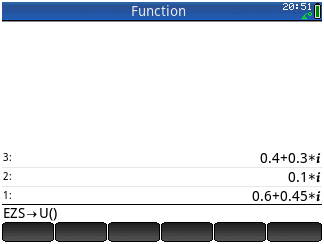
\includegraphics{Cap-CalcBas-EZS-HPP1.png}

    \item Premem a continuació la tecla 
\includegraphics{HPPrime-Enter.pdf} i la calculadora ens dona el valor de la tensió $\cmplx{U}$.

        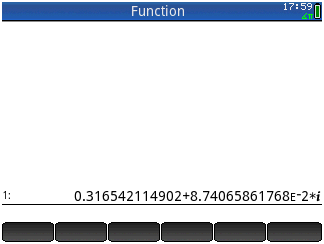
\includegraphics{Cap-CalcBas-EZS-HPP2.png}


     \item   Si la calculadora estigués en el mode \funsfbs{Algebraic} o en el mode  \funsfbs{Textbook}, escriuríem directament: \funsfbs{EZS\_U(0.4+0.3*i,0.1*i,0.6+0.45*i)}, i després de prémer la tecla 
\includegraphics{HPPrime-Enter.pdf} la calculadora ens donaria el valor de la tensió $\cmplx{U}$.

        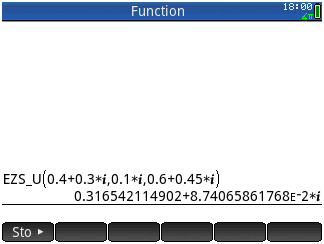
\includegraphics{Cap-CalcBas-EZS-HPP3.png}

    \end{dingautolist}
\end{exemple}



\section{Corrent de curtcircuit en el  secundari d'un transformador}
\index{corrent de curtcircuit!en el  secundari d'un transformador}\label{sec:cc-sec-trafo}

 Es tracta en aquest apartat el càlcul del corrent de curtcircuit trifàsic en el secundari d'un transformador que té el
primari connectat  a una xarxa de potència.

A partir de la Figura \vref{pic:cc_sec_trafo}, es tracta de trobar
el valor del corrent de curtcircuit trifàsic $I\ped{F}$ en el punt
F, essent la resta de paràmetres valors coneguts.

\begin{center}
    \input{Imatges/Cap-CalcBas-Icc-Trafo.pdf_tex}
    \captionsetup{justification=raggedright,margin={4cm,4cm},oneside}
    \captionof{figure}{Corrent de curtcircuit en el  secundari d'un
transformador} \label{pic:cc_sec_trafo}
\end{center}

$U\ped{N}$, $U\ped{TN1}$ i $U\ped{TN2}$ estan donats en volt,
$S\ped{cc}$ i $S\ped{TN}$ en voltampere, i $x\ped{cc}$ en per unitat
respecte dels valors nominals del transformador.


Per tal de simplificar el problema, suposarem que tant la impedància
de curtcircuit del transformador com la impedància equivalent de
la xarxa de potència són totalment inductives; d'aquesta manera
podrem treballar amb les diverses variables implicades com si
fossin nombres reals. Suposarem a més que no hi ha circulació de
corrent abans del curtcircuit.

Pel que fa a la xarxa de potència, si en lloc de la potència de curtcircuit $S\ped{cc}$, el que coneixem és el corrent de curtcircuit
disponible $I\ped{cc}$, podem obtenir el valor de la potència de
curtcircuit a partir de l'expressió:
\begin{equation}
    S\ped{cc} = \sqrt{3} U\ped{N} I\ped{cc}
\end{equation}
\index{potència de curtcircuit}

 Si prenem com a valors base els
paràmetres del transformador ($U\ped{TN1}$, $U\ped{TN2}$ i
$S\ped{TN}$), la relació de transformació i la impedància de curtcircuit del transformador, expressats en per unitat, seran 1:1 i
$x\ped{cc}$ respectivament. Anàlogament, la tensió i la impedància
equivalents de la xarxa de potència, expressats en per unitat, seran
$\frac{U\ped{N}}{U\ped{TN1}}$ i $\frac{U\ped{N}^2}{S\ped{cc}}
\frac{S\ped{TN}}{U\ped{TN1}^2}$ respectivament.

Amb aquests valors, el corrent de curtcircuit $i\ped{F}$, expressat
en per unitat, val:

\begin{equation}
    i\ped{F} = \frac{\dfrac{U\ped{N}}{U\ped{TN1}}}{\dfrac{U\ped{N}^2}{S\ped{cc}}
    \dfrac{S\ped{TN}}{U\ped{TN1}^2} + x\ped{cc}}
\end{equation}

I per tant, aquest corrent $I\ped{F}$ expressat en ampere, val:

\begin{equation}
    I\ped{F} = i\ped{F}\; \frac{S\ped{TN}}{\sqrt{3}U\ped{TN2}} =
    \frac{S\ped{TN} U\ped{N}}{\sqrt{3} U\ped{TN1}U\ped{TN2}
    \left(\dfrac{U\ped{N}^2}{S\ped{cc}}
    \dfrac{S\ped{TN}}{U\ped{TN1}^2} + x\ped{cc}\right)}
\end{equation}

Si la xarxa de potència es considera de potència infinita, tenim:

\begin{equation}
    I\ped{F} = \frac{S\ped{TN} U\ped{N}}{\sqrt{3} U\ped{TN1}U\ped{TN2}
    x\ped{cc}}\qquad\qquad (\text{amb }S\ped{cc}=\infty)
\end{equation}

Si a més, la tensió de la xarxa coincideix amb la tensió primària
del transformador, tenim respectivament:
\begin{align}
    I\ped{F} &= \frac{S\ped{TN}}{\sqrt{3} U\ped{TN2}
    \left(\dfrac{S\ped{TN}}{S\ped{cc}} +
    x\ped{cc}\right)}\qquad\qquad(\text{amb }U\ped{N}=U\ped{TN1})\\[1ex]
    I\ped{F} &= \frac{S\ped{TN}}{\sqrt{3} U\ped{TN2}
    x\ped{cc}}\qquad\qquad(\text{amb }U\ped{N}=U\ped{TN1}\text{ i }
    S\ped{cc}=\infty)
\end{align}

\addcontentsxms{Corrent de curtcircuit en el secundari d'un transformador}
\begin{exemple}[Corrent de curtcircuit en el secundari d'un transformador]
    A partir de la Figura \vref{pic:cc_sec_trafo}, amb els valors
    $U\ped{N}=\SI{6900}{V}$, $U\ped{TN1}=\SI{6900}{V}$,
    $U\ped{TN2}=\SI{400}{V}$, $S\ped{TN}=\SI{850}{kVA}$ i
    $x\ped{cc}=\SI{5}{\percent}$, es tracta de trobar $I\ped{F}$ en el cas
    que: a) $S\ped{cc}=\SI{200}{MVA}$ i b) $S\ped{cc}=\infty$.

    El valors demanats són:
    \begin{align*}
       &a)\;I\ped{F} = \frac{\SI{850}{kVA}}{\sqrt{3}\times \SI{400}{V}\times
       \left(\dfrac{\SI{850}{kVA}}{\SI{200}{MVA}} +
       \num{0,05}\right)} = \SI{22,6}{kA} \\[2ex]
       &b)\;I\ped{F} = \frac{\SI{850}{kVA}}{\sqrt{3}\times \SI{400}{V}\times
       \num{0,05}} = \SI{24,5}{kA}
    \end{align*}

\end{exemple}



\section{Escales logarítmiques}\label{sec:escales-log} \index{escales logarítmiques}

\subsection{Determinació de punts d'una corba}\index{escales logarítmiques!determinació de punts d'una corba}

En diferents camps de l'electrotècnia és usual trobar gràfics amb escales
logarítmiques.

Un exemple clar són els gràfics d'actuació dels interruptors magnetotèrmics o dels
fusibles, on les seves corbes característiques corrent--temps estan representades en
una escala logarítmica--logarítmica o lineal--logarítmica.

En aquests casos es presenta freqüentment la necessitat de determinar amb exactitud un
punt de la corba que no coincideix amb cap de les línies divisòries del gràfic. Atenent a
la Figura \vref{pic:escala log}, es tractaria de determinar el valor $x$ dins de la dècada
$10^N$ a $10^{N+1}$.

\begin{center}
    \input{Imatges/Cap-CalcBas-EscalesLog.pdf_tex}
    \captionof{figure}{Escala logarítmica}
    \label{pic:escala log}
\end{center}

Si mesurem amb un regle la distància $D$ des de l'inici de la dècada fins al punt $x$, i
la longitud total $L$ de la dècada, el valor $x$ buscat ve donat per l'expressió:

\begin{equation}
    x = 10^{\left(N+\frac{D}{L}\right)}
\end{equation}

Si estem interessats en el problema invers, és a dir, en  trobar la distància $D$
corresponent a un valor conegut $x$ dins de la dècada $10^N$ a $10^{N+1}$, podem emprar
l'expressió:

\begin{equation}
    D = L(\log x - N) = L \log\frac{x}{10^N}
\end{equation}

\addcontentsxms{Càlcul de valors en una escala logarítmica}
\begin{exemple}[Càlcul de valors en una escala logarítmica]
    Es tracta de trobar en primer lloc el valor $x$ dins de la dècada 100 a 1000, corresponent a una
    distància $D=\SI{11}{mm}$, i en segon lloc la distància $D$ a la qual hem de representar el valor $x=5$, dins de la
    dècada 1 a 10. La longitud total d'una dècada és $L=\SI{56}{mm}$.

    En el primer cas tenim $N=2$, i per tant:
    \[
        x = 10^{\left(2+\frac{\SI{11}{mm}}{\SI{56}{mm}}\right)}= \num{157,19}
    \]

    En el segon cas tenim $N=0$, i per tant:
    \[
        D = \SI{56}{mm} \times (\log 5 - 0)  = \SI{39,1}{mm}
    \]

\end{exemple}

\subsection{Determinació dels paràmetres d'una funció representada com una recta}\label{sec:escales-log-yxnk}\index{escales logarítmiques!determinació dels paràmetres d'una funció representada com una recta}

Quan la relació entre dues variables $y=f(x)$ compleix l'equació: $y x^n = k$, on $n$ i $k$  són constants  reals, la gràfica d'aquesta funció pren la forma d'una línia recta quan es representa en una escala logarítmica--logarítmica. Partint de l'equació inicial $y x^n = k$, si passem la variable $x$ a la dreta tenim:
\begin{equation}
  y = k x^{-n}
\end{equation}

Prenent logaritmes a banda i banda, tenim:
\begin{equation}
  \log y = \log k - n \log x
\end{equation}

Aquesta és l'equació d'una recta de pendent negatiu $n$, amb les variables $\log y$ i $\log x$.

A partir de la gràfica d'una recta en una escala logarítmica--logarítmica, podem determinar-ne les constants $n$ i $k$ seguint els passos següents:

\begin{dingautolist}{'312}
    \item Per  determinar el pendent $n$, només cal mesurar directament sobre la gràfica amb un regle, una distància horitzontal $\Delta{}x$ i una de vertical $\Delta{}y$ que partint d'un punt de la recta ens portin a un altre punt de la mateixa recta; a partir d'aquests dos valors, tenim:
        \begin{equation}
          n = \frac{\Delta{}y}{\Delta{}x}
        \end{equation}

        Aquesta equació suposa que la gràfica té una relació d'aspecte de 1:1, és a dir, que una dècada vertical i una d'horitzontal tenen la mateixa llargada. Si, per exemple, les dècades verticals tinguessin la meitat de la llargada que les dècades  horitzontals, caldria multiplicar per 2 el valor mesurat de $\Delta{}y$.

   \item  Un cop  coneixem $n$, a partir d'un punt qualsevol $(x_1, y_1)$ de la recta, podem calcular $k$ utilitzant l'equació inicial $y x^n = k$:
        \begin{equation}
          k =  y_1 x_1^n
        \end{equation}

        En el cas particular de $x_1=1$, l'equació anterior se simplifica a:\begin{equation}
           k = y_1\quad (\text{amb }x_1=1)
        \end{equation}
\end{dingautolist}

Aquest tipus de relació es compleix, per exemple en el cas dels cables elèctrics, entre el corrent de curtcircuit i el temps que el cable pot aguantar aquest corrent sense malmetre's. Vegeu la secció \vref{ces:cables_Icc_termica}.

\addcontentsxms{Càlcul de les constants $n$ i $k$ en una escala logarítmica--logarítmica}
\begin{exemple}[Càlcul de les constants $n$ i $k$ en una escala logarítmica--logarítmica]
    Es tracta de trobar les constants $n$ i $k$ de la funció que apareix dibuixada com una recta en la gràfica de la pàgina següent.

     Donat que la gràfica té una relació d'aspecte 1:1, a partir dels valors mesurats $\Delta{}y$ i $\Delta{}x$, tenim:
    \[
        n = \frac{\SI{171,6}{mm}}{\SI{57,2}{mm}} = 3
    \]

    Partint, per exemple, del valor d'abscisses: $x_1=100$, veiem que el valor corresponent d'ordenades és: $y_1=2$, i per tant tenim:
    \[
        k = 2 \times 100^3  = \num{2000000}
    \]

    L'equació que segueix aquesta funció, és doncs:
    \[
        y x^3 = \num{2000000}
    \]

   \begin{center}
        % GNUPLOT: LaTeX picture with Postscript
\begingroup
  \makeatletter
  \providecommand\color[2][]{%
    \GenericError{(gnuplot) \space\space\space\@spaces}{%
      Package color not loaded in conjunction with
      terminal option `colourtext'%
    }{See the gnuplot documentation for explanation.%
    }{Either use 'blacktext' in gnuplot or load the package
      color.sty in LaTeX.}%
    \renewcommand\color[2][]{}%
  }%
  \providecommand\includegraphics[2][]{%
    \GenericError{(gnuplot) \space\space\space\@spaces}{%
      Package graphicx or graphics not loaded%
    }{See the gnuplot documentation for explanation.%
    }{The gnuplot epslatex terminal needs graphicx.sty or graphics.sty.}%
    \renewcommand\includegraphics[2][]{}%
  }%
  \providecommand\rotatebox[2]{#2}%
  \@ifundefined{ifGPcolor}{%
    \newif\ifGPcolor
    \GPcolortrue
  }{}%
  \@ifundefined{ifGPblacktext}{%
    \newif\ifGPblacktext
    \GPblacktexttrue
  }{}%
  % define a \g@addto@macro without @ in the name:
  \let\gplgaddtomacro\g@addto@macro
  % define empty templates for all commands taking text:
  \gdef\gplbacktext{}%
  \gdef\gplfronttext{}%
  \makeatother
  \ifGPblacktext
    % no textcolor at all
    \def\colorrgb#1{}%
    \def\colorgray#1{}%
  \else
    % gray or color?
    \ifGPcolor
      \def\colorrgb#1{\color[rgb]{#1}}%
      \def\colorgray#1{\color[gray]{#1}}%
      \expandafter\def\csname LTw\endcsname{\color{white}}%
      \expandafter\def\csname LTb\endcsname{\color{black}}%
      \expandafter\def\csname LTa\endcsname{\color{black}}%
      \expandafter\def\csname LT0\endcsname{\color[rgb]{1,0,0}}%
      \expandafter\def\csname LT1\endcsname{\color[rgb]{0,1,0}}%
      \expandafter\def\csname LT2\endcsname{\color[rgb]{0,0,1}}%
      \expandafter\def\csname LT3\endcsname{\color[rgb]{1,0,1}}%
      \expandafter\def\csname LT4\endcsname{\color[rgb]{0,1,1}}%
      \expandafter\def\csname LT5\endcsname{\color[rgb]{1,1,0}}%
      \expandafter\def\csname LT6\endcsname{\color[rgb]{0,0,0}}%
      \expandafter\def\csname LT7\endcsname{\color[rgb]{1,0.3,0}}%
      \expandafter\def\csname LT8\endcsname{\color[rgb]{0.5,0.5,0.5}}%
    \else
      % gray
      \def\colorrgb#1{\color{black}}%
      \def\colorgray#1{\color[gray]{#1}}%
      \expandafter\def\csname LTw\endcsname{\color{white}}%
      \expandafter\def\csname LTb\endcsname{\color{black}}%
      \expandafter\def\csname LTa\endcsname{\color{black}}%
      \expandafter\def\csname LT0\endcsname{\color{black}}%
      \expandafter\def\csname LT1\endcsname{\color{black}}%
      \expandafter\def\csname LT2\endcsname{\color{black}}%
      \expandafter\def\csname LT3\endcsname{\color{black}}%
      \expandafter\def\csname LT4\endcsname{\color{black}}%
      \expandafter\def\csname LT5\endcsname{\color{black}}%
      \expandafter\def\csname LT6\endcsname{\color{black}}%
      \expandafter\def\csname LT7\endcsname{\color{black}}%
      \expandafter\def\csname LT8\endcsname{\color{black}}%
    \fi
  \fi
    \setlength{\unitlength}{0.0500bp}%
    \ifx\gptboxheight\undefined%
      \newlength{\gptboxheight}%
      \newlength{\gptboxwidth}%
      \newsavebox{\gptboxtext}%
    \fi%
    \setlength{\fboxrule}{0.5pt}%
    \setlength{\fboxsep}{1pt}%
    \definecolor{tbcol}{rgb}{1,1,1}%
\begin{picture}(9060.00,12740.00)%
    \gplgaddtomacro\gplbacktext{%
      \colorrgb{0.00,0.00,0.00}%%
      \put(816,900){\makebox(0,0)[r]{\strut{} 0,1}}%
      \colorrgb{0.00,0.00,0.00}%%
      \put(816,4724){\makebox(0,0)[r]{\strut{} 1}}%
      \colorrgb{0.00,0.00,0.00}%%
      \put(816,8547){\makebox(0,0)[r]{\strut{} 10}}%
      \colorrgb{0.00,0.00,0.00}%%
      \put(816,12371){\makebox(0,0)[r]{\strut{} 100}}%
      \colorrgb{0.00,0.00,0.00}%%
      \put(997,603){\makebox(0,0){\strut{} 10}}%
      \colorrgb{0.00,0.00,0.00}%%
      \put(4821,603){\makebox(0,0){\strut{} 100}}%
      \colorrgb{0.00,0.00,0.00}%%
      \put(8645,603){\makebox(0,0){\strut{} 1000}}%
      \csname LTb\endcsname%%
      \put(824,5875){\makebox(0,0)[r]{\strut{}2}}%
    }%
    \gplgaddtomacro\gplfronttext{%
      \csname LTb\endcsname%%
      \put(504,6636){\makebox(0,0){\strut{}$y$}}%
      \csname LTb\endcsname%%
      \put(8698,6636){\rotatebox{-270}{\makebox(0,0){\strut{}}}}%
      \csname LTb\endcsname%%
      \put(4821,284){\makebox(0,0){\strut{}$x$}}%
      \csname LTb\endcsname%%
      \put(4821,12371){\makebox(0,0){\strut{}}}%
      \csname LTb\endcsname%%
      \put(2647,7221){\rotatebox{-270}{\makebox(0,0){\strut{}$\Delta{}y =\qty{171,6}{mm}$}}}%
      \csname LTb\endcsname%%
      \put(3973,2171){\makebox(0,0){\strut{}$\Delta{}x =\qty{57,2}{mm}$}}%
      \csname LTb\endcsname%%
      \put(4821,12371){\makebox(0,0){\strut{}}}%
    }%
    \gplbacktext
    \put(0,0){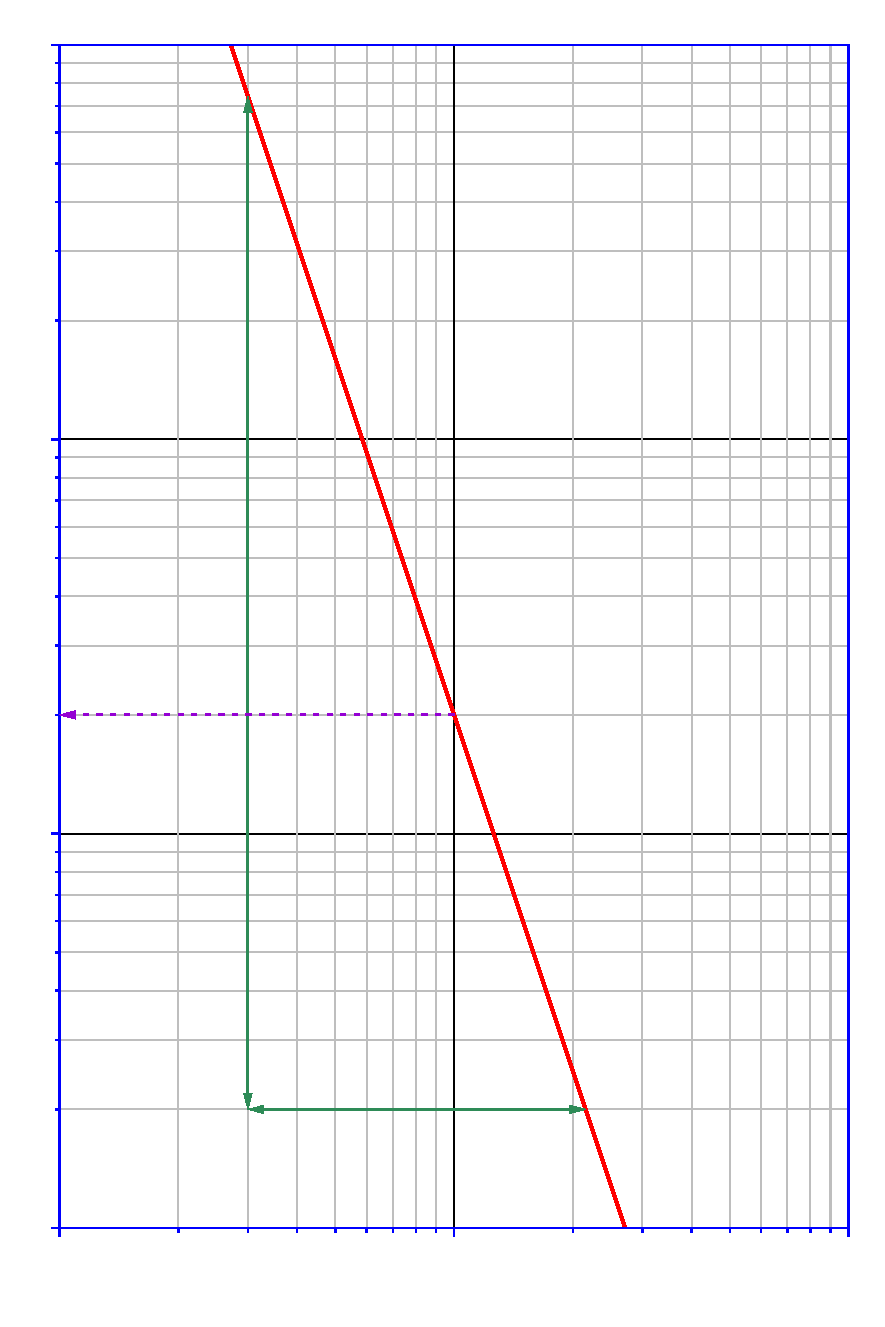
\includegraphics[width={453.00bp},height={637.00bp}]{Cap-CalcBas-RectaLogLog}}%
    \gplfronttext
  \end{picture}%
\endgroup

   \end{center}

\end{exemple}

